\newpage
\section{Tests}
\label{sec:tests}
This chapter presents the tests for the compiler. The development process was \emph{Test Driven Development} (TDD). This process is shown in the following figure \ref{fig:tdd}:

\begin{figure}[bth]
	\centering
	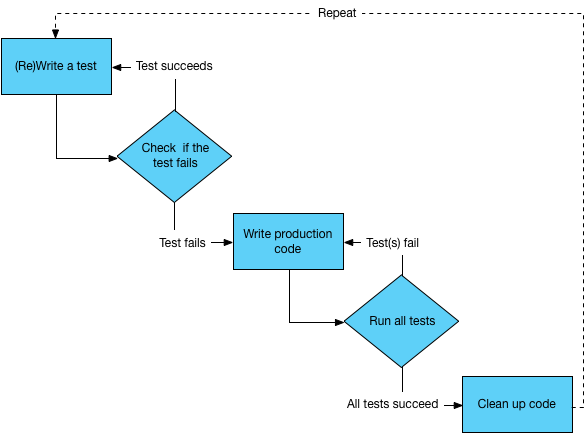
\includegraphics[scale=0.6]{./img/tdd}
	\caption[Test Driven Development]{Test Driven Development}
	\label{fig:tdd}
\end{figure}
\noindent

Test cases were created as early as possible and derived from desired use cases of the compiler. Furthermore, they specified the preconditions and the behavior of the respective product functions. If the parser did not throw any more mistakes, then the grammar was correct. However, a \texttt{NoSuchElementException} indicated that the instruction code was still produced incorrectly. Therefore, the test drivers were developed first whereby methods were partially defined at the beginning.

The unit and integration tests serve to exclude errors of the calculated results. TestNG\footnote{TestNG, \url{https://testng.org/doc/index.html}} was used as test framework. It is inspired by JUnit\footnote{JUnit, \url{https://junit.org/junit5/}} but is easier to use and offers more functionalities like annotations or a flexible test configuration. The test suite is structured as follows (see code \ref{lst:compiler_test}):

\begin{lstlisting}[frame=htrbl, caption={Implementation of {\ttfamily CompilerTest.java}}, label={lst:compiler_test}, basicstyle=\footnotesize]
public class CompilerTest {
   @BeforeClass
   public void createTempDir() throws Exception {
      Main.tempDir = Main.createTempDir("compilerTest");
   }

   @AfterClass
   public void deleteTempDir() {
      Main.deleteRecursive(Main.tempDir.toFile());
   }

   @DataProvider
   public Object[][] provideCodeExpectedOutput() {
      return new Object[][] {
         {"Print a number", "print(1);", "1"},
         {"Print a number with a new line", "println(1);", "1" + 
            System.lineSeparator()},
         {"Addition", "print(1+2);", "3"},
         {"Chained addition", "print(1.0+2.3+50.8);", "54.1"},
         {"Subtraction", "print(5-3);", "2"},
         {"Multiplication", "print(2*5);", "10"},
         {"Division", "print(9/3);", "3"},
         {"Integer division", "print(10/3);", "3"},
         {"Floating point number division", "print(7.0/2.0);", "3.5"},
         {"Modulo", "print(12%5);", "2"},
         {"Division and multiplication", "print(15/5*3);", "9"},
         {"Subtraction and addition", "print(3-2+5);", "6"},
         {"Addition and subtraction", "print(3+2-5);", "0"},
         {"Order of operations", "print(9-1*3);", "6"},
         {"Order of operations 2", "print(3+5*2);", "13"},
         {"Multiple output", "println(1); println(2);", "1" + 
            System.lineSeparator() + "2" + System.lineSeparator()},
         {"Variable declaration", "int a; a = 5; print(a);", "5"},
         {"Variable declaration 2", "int _a; _a = 5; print(_a);", "5"},
         {"Variable declaration and constant", "int a; a = 5; 
            print(a+3);", "8"},
         {"Variable declaration and calculation", "int a; a = 5; 
            int b; b = 3; print(a+b);", "8"},
         loadTestCode("function/simple", "3"),
         loadTestCode("function/local_parameter", "3"),
         loadTestCode("function/scope", "3" + System.lineSeparator() + 
            "5"),
         loadTestCode("function/current_formal_parameter", "15"),
         loadTestCode("function/overloading", "1" + 
            System.lineSeparator() + "5"),
         loadTestCode("branch/if-else_zero_false", "1"),
         loadTestCode("branch/if-else_one_true", "1"),
         loadTestCode("branch/if-else_other_true", "1"),
         {"Lower than to true", "print(0 < 1);", "1"},
         {"Lower than to false", "print(2 < 2);", "0"},
         {"Lower than to false 2", "print(3 < 2);", "0"},
         {"Lower than/equal to true", "print(0 <= 1);", "1"},
         {"Lower than/equal to true 2", "print(2 <= 2);", "1"},
         {"Lower than/equal to false", "print(3 <= 2);", "0"},
         {"Greater than to true", "print(1 > 0);", "1"},
         {"Greater than to false", "print(2 > 2);", "0"},
         {"Greater than to false 2", "print(1 > 2);", "0"},
         {"Greater than/equal to true", "print(1 >= 0);", "1"},
         {"Greater than/equal to true 2", "print(2 >= 2);", "1"},
         {"Greater than/equal to false", "print(0 >= 1);", "0"},
         {"Negation", "print(3 * -5);", "-15"},
         {"Logical conjunction to true", "print(1 && 1);", "1"},
         {"Logical conjunction to false", "print(0 && 1);", "0"},
         {"Logical conjunction to false 2", "print(1 && 0);", "0"},
         {"Logical conjunction to false 3", "print(0 && 0);", "0"},
         {"Logical disjunction to true", "print(1 || 1);", "1"},
         {"Logical disjunction to true 2", "print(0 || 1);", "1"},
         {"Logical disjunction to true 3", "print(1 || 0);", "1"},
         {"Logical disjunction to false", "print(0 || 0);", "0"},
         loadTestCode("operators/lazy_eval_and", "0" + 
            System.lineSeparator() + "0"),
         loadTestCode("operators/lazy_eval_or", "1" + 
            System.lineSeparator() + "1"),
         {"Logical contravalence to true", "print(0 ^ 1);", "1"},
         {"Logical contravalence to true 2", "print(1 ^ 0);", "1"},
         {"Logical contravalence to false", "print(0 ^ 0);", "0"},
         {"Logical contravalence to false 2", "print(0 ^ 0);", "0"},
         {"Print string literal", "print(\"Hello world\");", 
            "Hello world"},
         {"Print string literal 2", "String a = \"Hello world\"; 
            print(a);", "Hello world"},
         loadTestCode("comments/line_comment", "5"),
         loadTestCode("comments/multiline_comment", "5"),
         loadTestCode("comments/special_comment", "5"),
         loadTestCode("loop/while", "4"),
         {"Casting to integer", "print(toInt(5.3));", "5"},
         {"Casting to float", "print(toFloat(\"3\"));", "3.0"},
         {"Casting to string", "String a = toString(5.0); print(a);", 
            "5.0"},
         {"Append characters", "String a = append(\"a\", \"b\"); 
            print(a);", "ab"},
         loadTestCode("assembly/inline_asm", "5.5"),
         {"Access to an array", "int[] a = new int[3]; a[0] = 5; 
            print(a[0]);", "5"},
         {"Print array length", "int[] a = new int[3]; print(length(a)
            );", "3"}
      };
   }
   
   private static String[] loadTestCode(final String filePath, 
      final String expectedResult) throws Exception {
      try (InputStream input = CompilerTest.class.getResourceAsStream(
         "/" + filePath + ".e")) {
         if (input == null) {
            throw new IllegalArgumentException("The file " + filePath + 
               ".e does not exist");
         }
         String code = new Scanner(input).useDelimiter("\\A").next();
         return new String[]{filePath, code, expectedResult};
      }
   }

   @Test(dataProvider = "provideCodeExpectedOutput")
   public void testOutputs(final String description, final String 
      sourceCode, final String expectedOutput) throws Exception {
      final String currentOutput = compileAndRun(sourceCode);
      Assert.assertEquals(currentOutput, expectedOutput);
   }
   
   @Test(expectedExceptions = UndeclaredVariableException.class,
      expectedExceptionsMessageRegExp = "1:6 Undeclared variable: <a>;")
   public void testReadingUndeclaredVariable() throws Exception {
      compileAndRun("print(a);");
   }
   
   @Test(expectedExceptions = UndeclaredVariableException.class,
      expectedExceptionsMessageRegExp = "1:0 Undeclared variable: <a>;")
   public void testWritingUndeclaredVariable() throws Exception {
      compileAndRun("a = 9;");
   }
   
   @Test(expectedExceptions = AlreadyDefinedVariableException.class,
      expectedExceptionsMessageRegExp = "2:4 Already defined variable: 
      <a>;")
   public void testWritingAlreadyDefinedVariable() throws Exception {
      compileAndRun("int a;" + System.lineSeparator() + "int a;");
   }
   
   @Test(expectedExceptions = UndefinedFunctionException.class,
      expectedExceptionsMessageRegExp = "1:6 Undefined function: 
      <foo>;")
   public void testReadingUndefinedFunction() throws Exception {
      compileAndRun("print(foo());");
   }
   
   @Test(expectedExceptions = AlreadyDefinedFunctionException.class,
      expectedExceptionsMessageRegExp = 
   "2:4 Already defined function: <get_val>;")
   public void testWritingAlreadyDefinedFunction() throws Exception {
      compileAndRun("int get_val() { return 1; }" + '\n' + 
         "int get_val()
         { return 2; }");
   }
   
   @Test(expectedExceptions = AlreadyDeclaredStructException.class,
      expectedExceptionsMessageRegExp = "2:7 Already declared struct: 
      <a>;" )
   public void testWritingAlreadyDeclaredStruct() throws Exception {
   compileAndRun("struct a { int a; }" + System.lineSeparator() + 
      "struct a { int b; }");
   }
   
   @Test(expectedExceptions = UndeclaredStructException.class,
      expectedExceptionsMessageRegExp = "1:11 Undeclared struct: 
      <Point>;")
   public void testReadingUndeclaredStruct() throws Exception {
      compileAndRun("struct a { Point p; }");
   }
   
   @Test(expectedExceptions = WrongDataTypeException.class,
      expectedExceptionsMessageRegExp = "1:8 Wrong data type: <3>;")
   public void testUsingWrongDataType() throws Exception {
      compileAndRun("int a = 3 + 5.0;");
   }
   
   @Test(
   expectedExceptions = UnknownModuleException.class,
      expectedExceptionsMessageRegExp = "1:6 The module could not be 
      found: <math>;")
   public void testUsingFunctionOfUnknownModule() throws Exception {
      compileAndRun("print(math.square(5): int);");
   }

   private String compileAndRun(final String sourceCode) throws 
      Exception {
      final String compiledCode = Main.compile(CharStreams
         .fromString(sourceCode));
      // System.out.println(sourceCode);
      final ClassFile classFile = new ClassFile();
      classFile.readJasmin(new StringReader(compiledCode), "", false);
      Path outputPath = Main.tempDir.resolve(classFile.getClassName() +
      ".class");
      try ( OutputStream output = Files.newOutputStream(outputPath) ) {
         classFile.write(output);
      }
      return runClass(Main.tempDir, classFile.getClassName());
   }
}
\end{lstlisting}

Before execution a temporary folder ``compilerTest'' is created by the method \\\texttt{createTempDir}. This folder is deleted via \texttt{deleteTempDir} or \texttt{deleteRecursive}. The test is annotated by \texttt{@test} where a data provider \texttt{provideCodeExpectedOutput} is registered. This holds the individual code snippets or components of the compiler (see code \ref{lst:pe} on page \pageref{lst:pe}) which are tested individually and continuously. The first string represents the description, the second the source code and the third the expected result. Since there are also longer constructs, these are loaded separately from files using the \texttt{loadTestCode} method. The individual files are listed in the appendix on page \pageref{sec:testfiles}. The error messages are also tested which is annotated by the expected exceptions. The current result is determined by the \texttt{compileAndRun} method. The corresponding compilation is created in the class \texttt{Main} (see code \ref{lst:main} on page \pageref{lst:main}). An excerpt of the tests can be seen in the figure \ref{fig:tests} below:

\begin{figure}[bth]
	\centering
	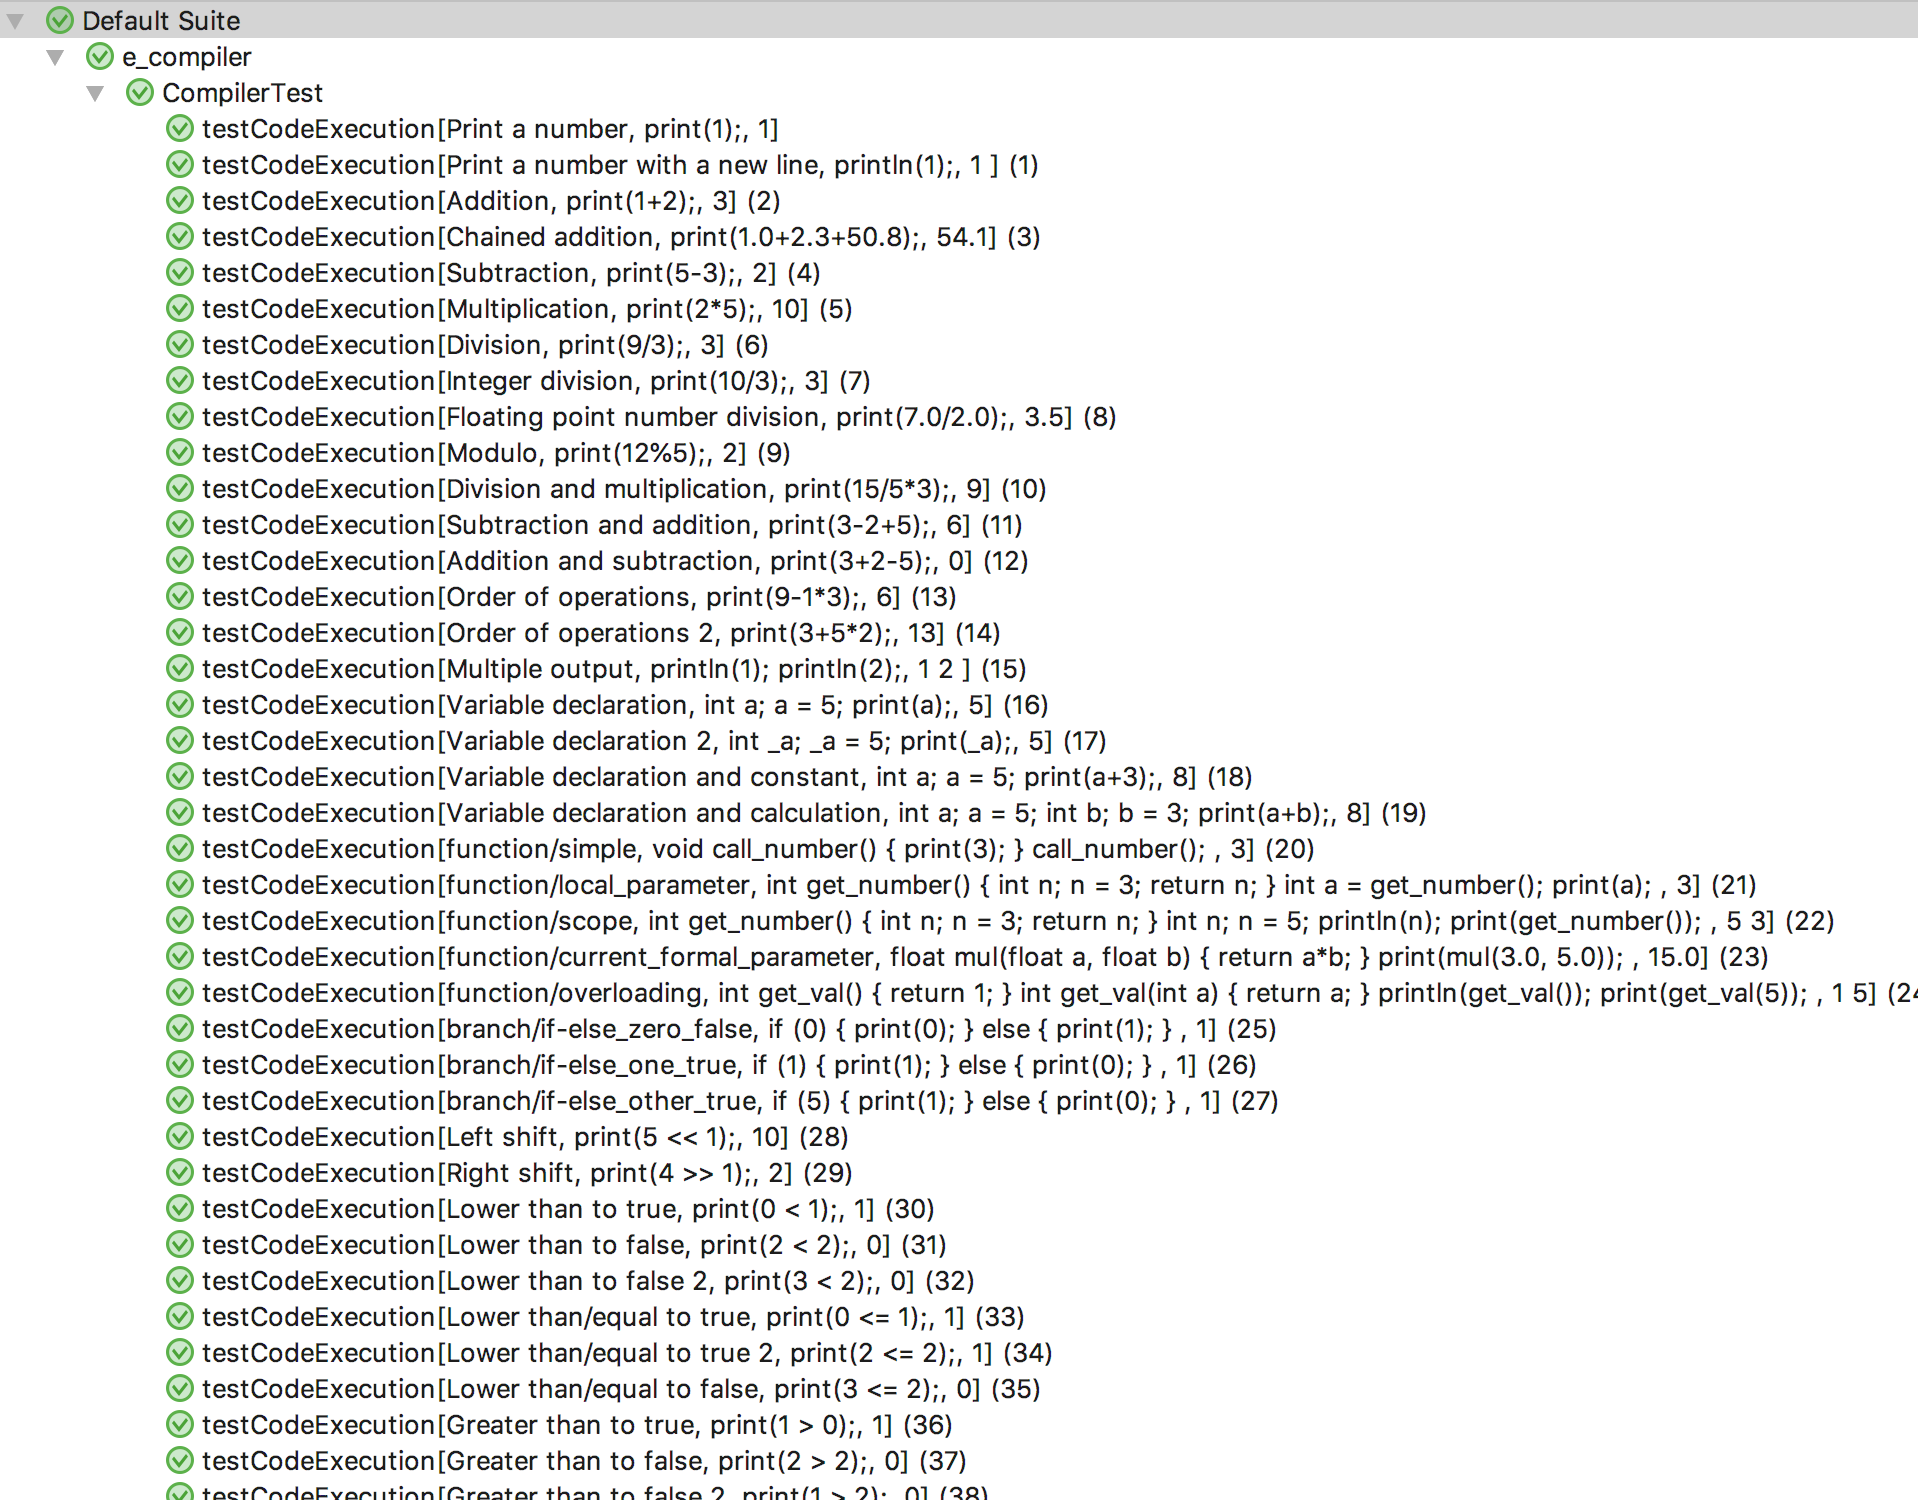
\includegraphics[scale=0.32]{./img/tests}
	\caption[Unit and integrations tests]{Unit and integrations tests}
	\label{fig:tests}
\end{figure}
\noindent

Accordingly, it can be recognized that all 83 tests regarding arithmetic operators, outputs, functions, variable declarations, loops, branches, structures etc. have been successful and that the compiler works correctly regarding language \emph{E}. To ensure the code quality, Google Java Format\footnote{Google Java Format, \url{https://github.com/google/google-java-format}} was still used which formats the code. Checkstyle\footnote{Checkstyle, \url{https://maven.apache.org/plugins/maven-checkstyle-plugin/}} was also used. It can find class design problems, method design problems. It also has the ability to check code layout and formatting issues.